\begin{sidewaysfigure*}
\thisfloatpagestyle{mylandscape}%
\rotatesidewayslabel%
\centering

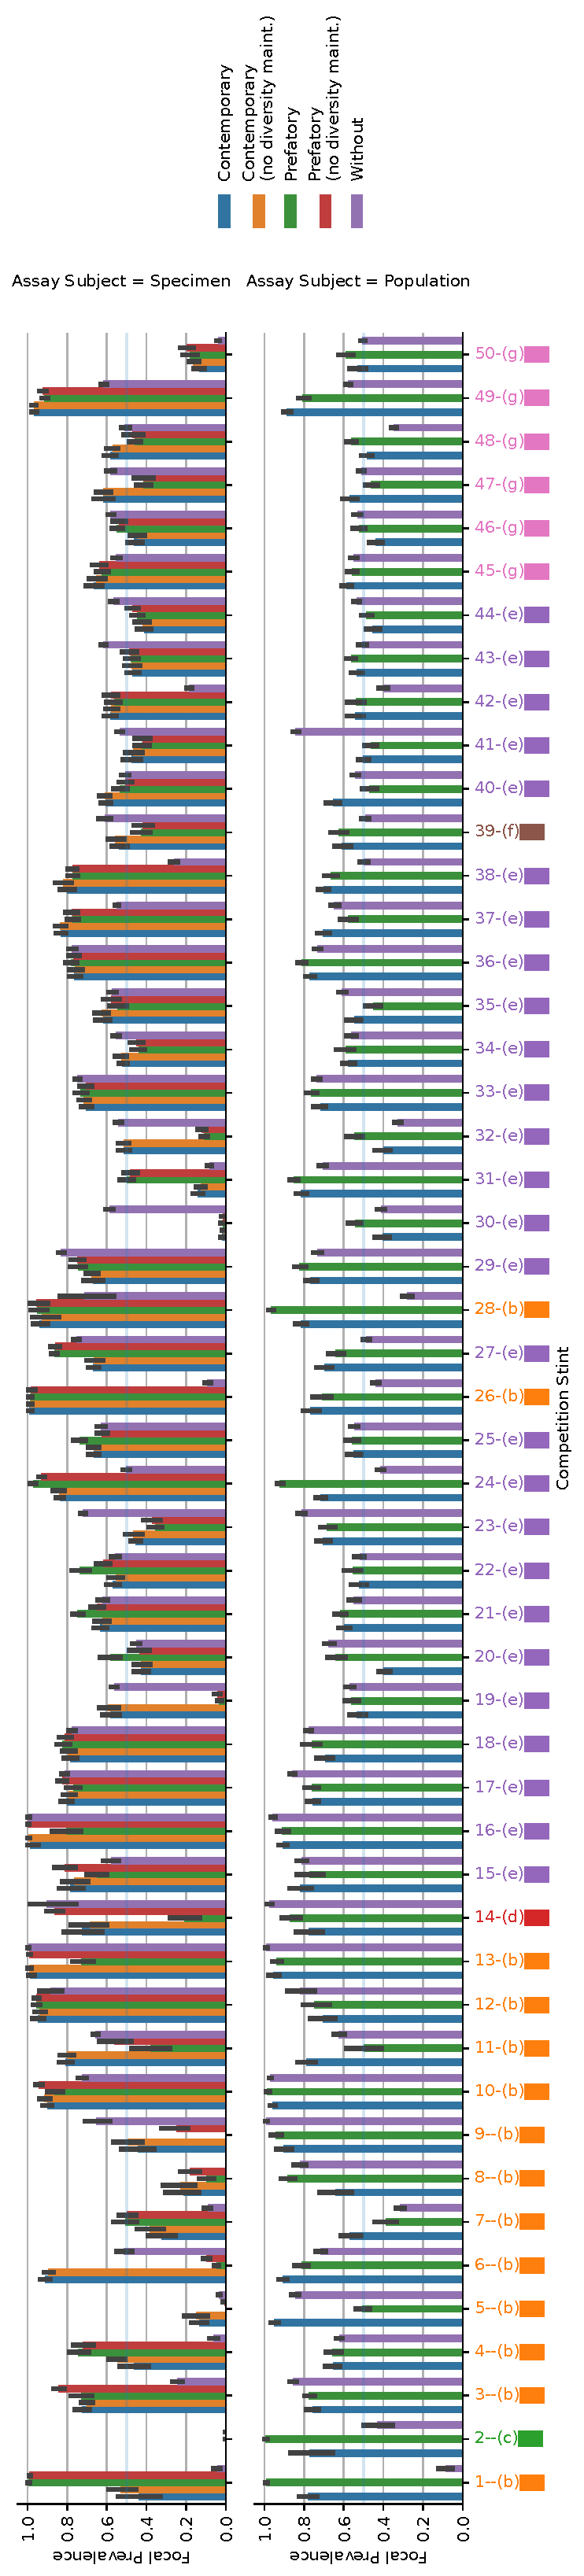
\includegraphics[width=\linewidth]{{submodule/dishtiny/binder/bucket=prq49/a=adaptation_assays+endeavor=16/teeplots/hue=biotic-background+stint=1-50+viz=facet-barplot+x=competition-stint+y=focal-prevalence+ext=}}

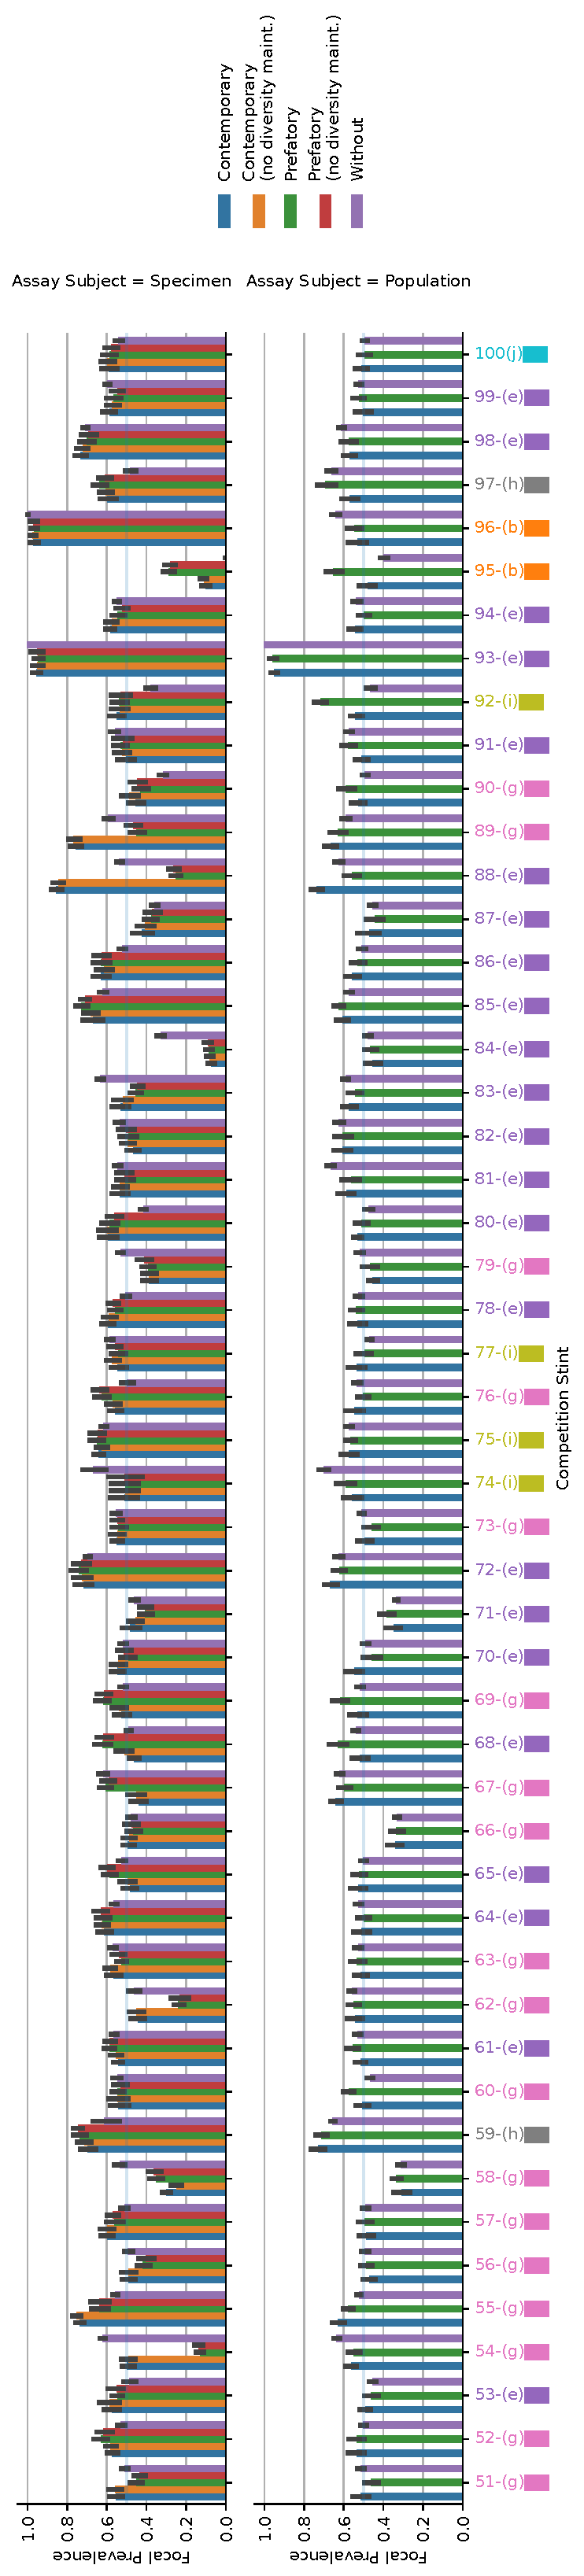
\includegraphics[width=\linewidth]{{submodule/dishtiny/binder/bucket=prq49/a=adaptation_assays+endeavor=16/teeplots/hue=biotic-background+stint=51-100+viz=facet-barplot+x=competition-stint+y=focal-prevalence+ext=}}

\caption{
End-state population composition of competition experiments.
Half (0.5) population composition corresponds to a neutral result.
Zero population composition corresponds to extreme fitness loss compared to the previous stint.
Population composition of 1.0 corresponds to extreme fitness gain compared to the previous stint.
Error bars are bootstrapped 95\% confidence intervals.
Color coding and parentheticals of stint labels correspond to qualitative morph codes described in Table \ref{tab:morph_descriptions}.
Upper panels show results for sampled focal strain genome, lower panels show results for entire focal strain population.
Figure is split into two rows due to layout considerations.
See Figure \ref{fig:adaptation_assay_cartoon} for explanation of competition biotic backgrounds.
See Figure \ref{fig:mean_competition_prevalence_boxplot} for boxplot depiction of prevalence outcomes.
}
\label{fig:mean_competition_prevalence_barplot}
\end{sidewaysfigure*}
